%!TeX program = xelatex

\documentclass[aspectratio=169]{beamer}
\usepackage[english]{babel}
\usepackage{fontspec}
\usepackage{graphicx}
\usepackage{xcolor}
\usepackage{xltxtra}
\usepackage{hyperref}
\usepackage{multicol}
\usepackage{unicode-math}
\usepackage{changepage}
\usepackage{tcolorbox}

\usetheme{Warsaw}
\setbeamertemplate{navigation symbols}{}
\setbeamertemplate{headline}{}
\setbeamertemplate{bibliography item}[text]

\definecolor{MainRed}{RGB}{175,44,34}     % CMYK 3-95-94-29
\definecolor{DarkRed}{RGB}{127,37,2}      % CMYK 22-91-82-46
\definecolor{AltRed}{RGB}{150,40,14}

\definecolor{GoldLight}{RGB}{200,160,110} % CMYK 18-35-60-10
\definecolor{GoldDark}{RGB}{150,121,82}   % CMYK 18-35-60-40

\definecolor{GrayOne}{RGB}{198,198,198}
\definecolor{GrayTwo}{RGB}{160,160,160}
\definecolor{GrayThr}{RGB}{135,135,135}

\definecolor{NearBlack}{RGB}{31,31,31}

\definecolor{Bejevi}{RGB}{201,188,171}
\definecolor{NearWhite}{RGB}{227,227,227}

\setbeamercolor{structure}{fg=MainRed}
\setbeamercolor{palette primary}{fg=white,bg=DarkRed}
\setbeamercolor{palette secondary}{fg=white,bg=MainRed}
\setbeamercolor{palette tertiary}{fg=white,bg=DarkRed}
\setbeamercolor{palette quaternary}{fg=white,bg=MainRed}

\setbeamercolor{title}{fg=white,bg=MainRed}
\setbeamercolor{frametitle}{fg=white,bg=MainRed}
\setbeamercolor{titlelike}{fg=white,bg=MainRed}

\setbeamercolor{normal text}{fg=black,bg=white}

\setbeamercolor{block title}{fg=white,bg=DarkRed}
\setbeamercolor{block body}{fg=black,bg=DarkRed!8}

\setbeamercolor{block title alerted}{fg=white,bg=MainRed}
\setbeamercolor{block body alerted}{fg=black,bg=MainRed!10}

\setbeamercolor{block title example}{fg=white,bg=GoldDark}
\setbeamercolor{block body example}{fg=black,bg=GoldLight!20}

\setbeamercolor{title in head/foot}{fg=white,bg=DarkRed}
\setbeamercolor{author in head/foot}{fg=white,bg=NearBlack}
\setbeamercolor{date in head/foot}{fg=white,bg=GrayTwo}

\setbeamertemplate{footline}{
        \leavevmode%
        \hbox{%
                \begin{beamercolorbox}[wd=.72\paperwidth,ht=2.8ex,dp=1.2ex,leftskip=1em]{title
                        in head/foot}%
                        \insertshorttitle
                \end{beamercolorbox}%
                \begin{beamercolorbox}[wd=.14\paperwidth,ht=2.8ex,dp=1.2ex,center]{author
                        in head/foot}%
                        Shago P. E.
                \end{beamercolorbox}%
                \begin{beamercolorbox}[wd=.14\paperwidth,ht=2.8ex,dp=1.2ex,center]{date
                        in head/foot}%
                        \insertframenumber/\inserttotalframenumber
                \end{beamercolorbox}%
        }%
        \vskip0pt%
}

\tcbuselibrary{skins}
\newtcolorbox{shadowbox}{
        enhanced,
        colback=GrayOne,
        colframe=white,
        boxrule=0pt,
        sharp corners=all,
        arc=6pt,
        drop shadow,
        left=4mm,
        right=4mm,
        top=2mm,
        bottom=2mm
}

\newtcolorbox{shadowbox2}{
        enhanced,
        colback=NearWhite,
        colframe=white,
        boxrule=0pt,
        arc=4pt,
        outer arc=4pt,
        fuzzy shadow={
        0mm}{-1.3mm}{0mm}{0.3mm}{black!30
        },
        coltext=NearBlack,
        halign=center,
        fontupper=\centering,
        left=4mm,
        right=4mm,
        top=2mm,
        bottom=2mm
}

\setmainfont{Iosevka NFM}
\setmonofont{Iosevka NFM}
\setsansfont{Iosevka NFM}
\setromanfont{Iosevka NFM Italic}
\setmathfont{Latin Modern Math}

\title{EEVDF Linux Process Scheduler implementation via sched\_ext}
\author{Shago Pavel Evgenevich}

\institute {
        Saint Petersburg State University\\
        \vspace{0.2cm}
        CPS 2026
}

\date{\small April 9}

\begin{document}

\begin{frame}
        \titlepage
\end{frame}

\begin{frame}{Introduction}
        \begin{shadowbox2}
                \small CPU scheduling is a core mechanism of OS
                process management

                \small OS scheduler governs how to allocate
                processor time among competing tasks
        \end{shadowbox2}
        \vspace{0.7em}

        \textbf{Linux Kernel}
        \begin{itemize}
                \item Open-source operating system kernel
                \item Manages hardware resources
                \item Widely used across computing domains
        \end{itemize}

        \vspace{0.5em}

        \textbf{The OS Scheduler}
        \begin{itemize}
                \item Subsystem for task selection and CPU allocation
                \item Determines execution order and task's time slicing
                \item Governs resource utilization, responsiveness,
                        and predictability
        \end{itemize}
\end{frame}

\begin{frame}{Problem}
        \begin{itemize}
                \item The built-in Linux EEVDF scheduler is part of
                        the kernel and cannot be modified without
                        recompilation and a full system reboot

                        \vspace{0.3em}
                \item This work investigates reimplementation of EEVDF
                        via sched\_ext to study how different implementation
                        approach can affect scheduling performance

                        \vspace{0.3em}
                \item To evaluate the implementation, standard
                        workload benchmarks are used such as
                        hackbench, sysbench, and eBPF-based
                        scheduling latency tracing

                        \vspace{0.3em}
                \item Then the sched\_ext variant is compared against
                        the built-in kernel EEVDF to identify
                        trade-offs introduced by eBPF dispatch
        \end{itemize}
\end{frame}

\begin{frame}{sched\_ext}
        \begin{shadowbox2}
                \small \textbf{sched\_ext} (scheduler extensions)
                is a new Linux kernel infrastructure that enabled
                implementing CPU scheduling policies as eBPF programs
                attached to kernel scheduling hooks at runtime
        \end{shadowbox2}

        \vspace{0.4em}
        \begin{columns}[T]
                \column{0.50\textwidth}
                \vspace{0.5em}
                \centering
                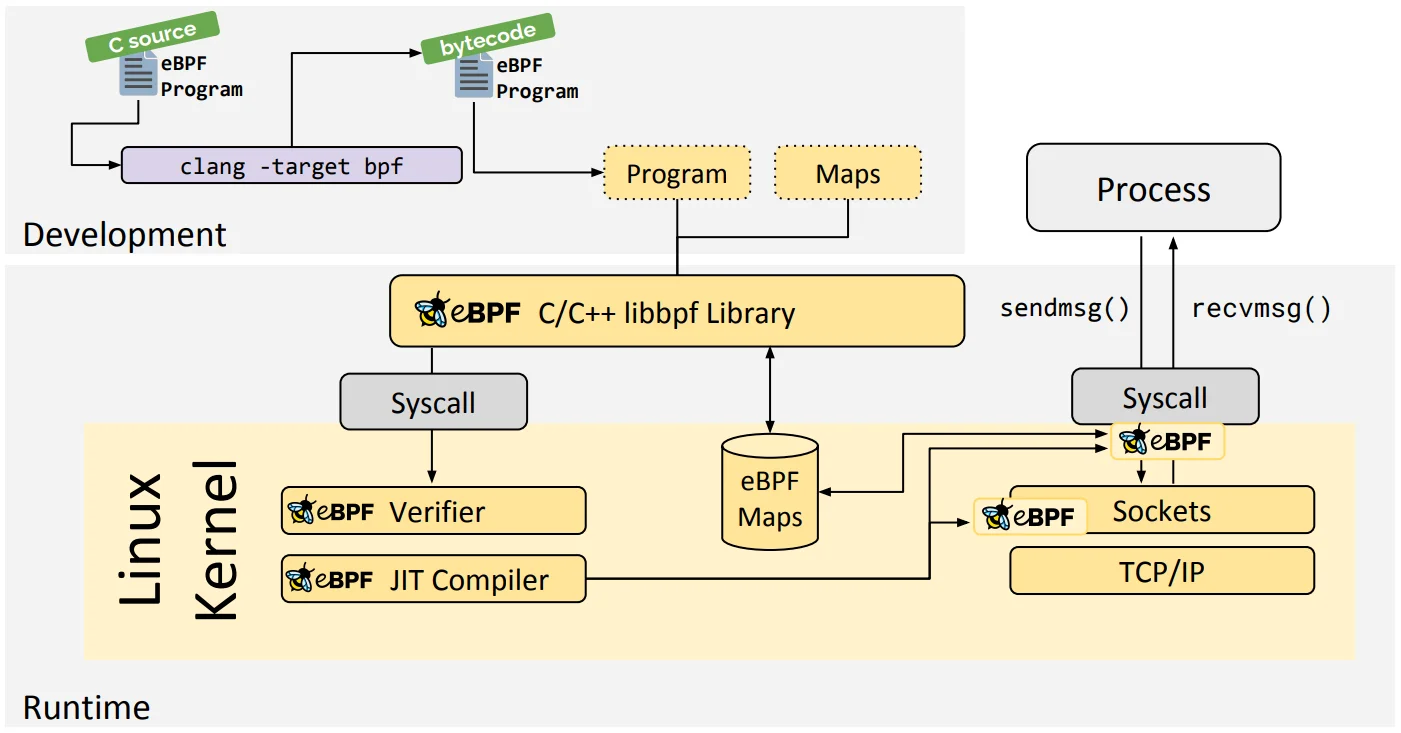
\includegraphics[width=\linewidth]{../0212/res/libbpf.png}

                \vspace{0.1em}
                {\tiny \textbf{Figure\ 1.} eBPF in the network subsystem}

                \column{0.50\textwidth}
                \textbf{DSQs} (dispatch queues):
                {\footnotesize
                        \begin{itemize}
                                \item \texttt{SCX\_DSQ\_LOCAL} --
                                        per-core fast path
                                \item \texttt{SCX\_DSQ\_GLOBAL} -- shared queue
                \end{itemize}}


                \vspace{0.2em}
                \textbf{Scheduler cycle:}
                {\footnotesize
                        \begin{itemize}
                                \item \texttt{select\_cpu} -- pick idle cpu core
                                \item \texttt{enqueue} -- place task
                                        in global DSQ
                                \item \texttt{dispatch} -- move to local DSQ
                                \item \texttt{running} /
                                        \texttt{stopping} -- based on vtime
                \end{itemize}}

        \end{columns}
\end{frame}

\begin{frame}{Earliest Eligible Virtual Deadline First Model}
        The ideal reference system is such system where every active
        client $i$ continuously receives share $w_i / W(t)$ of the CPU.
        EEVDF tracks this entitlement through system virtual time $V(t)$,

        $$ W(t)=\sum_{j\in A(t)} w_j, \qquad
        V(t)=\int_{t_0}^{t}\frac{d\tau}{W(\tau)}.$$

        When client $i$ submits a request of size $r$, the algorithm
        assigns a \emph{virtual eligible time} and a \emph{virtual deadline},

        $$v_e = V(t_0^i)+\frac{s_i(t_0^i,t)}{w_i}, \qquad
        v_d = v_e + \frac{r}{w_i},$$

        where $s_i(t_0^i,t)$ is the service received since $t_0^i$.
\end{frame}

\begin{frame}{Earliest Eligible Virtual Deadline First Model}
        A request is runnable only once $v_e \le V(t)$. Among all
        eligible requests, EEVDF dispatches the one with the smallest
        virtual deadline $v_d$.

        \vspace{0.6em}

        A client behind its proportional share carries a smaller $v_e$
        and becomes eligible sooner. Larger weights compress $r/w_i$,
        so heavier tasks earn earlier deadlines for the same request size.

        \vspace{0.6em}

        \begin{shadowbox}
                The lag of client $i$ measures the signed deviation between
                ideal model entitlement and actual service received.
                EEVDF guarantees \cite{stoica} $|\mathrm{lag}_i(t)| <
                q$ in steady state,
                the optimal bound for any discrete proportional-share
                scheduler with quantum $q$.
        \end{shadowbox}
\end{frame}

\begin{frame}{Mapping to sched\_ext}
        \begin{columns}
                \column{0.42\textwidth}
                \begin{tabular}{ll}
                        Client  & $\to$ \texttt{task\_struct} \\[2pt]
                        $w_i$   & $\to$ \texttt{p->scx.weight} \\[2pt]
                        $v_i$   & $\to$ \texttt{scx.dsq\_vtime} \\[2pt]
                        $V(t)$  & $\to$ \texttt{vtime\_now} \\[2pt]
                        $r$     & $\to$ \texttt{SCX\_SLICE\_DFL}
                \end{tabular}

                \vspace{3.5em}
                {\footnotesize $ S $ --  integer scale}

                \column{0.58\textwidth}
                \textbf{enqueue:}
                $$VE_i = \max(v_i,\; V_\mathrm{now} - \Delta)$$
                $$VD_i = VE_i + \frac{r \cdot S}{w_i}
                \;\to\; \text{insert by } VD_i$$

                \textbf{running:}
                $$V_\mathrm{now} \leftarrow \max(V_\mathrm{now},\; v_i)$$

                \textbf{stopping:}
                $$v_i \leftarrow v_i +
                \frac{\mathrm{consumed}\cdot S}{w_i}$$
        \end{columns}
\end{frame}

\begin{frame}{Environment}
        \begin{columns}[T]
                \column{0.24\textwidth}
                \begin{shadowbox}
                        \small\textbf{System}

                        \vspace{0.25cm}
                        \footnotesize
                        Kernel:\\Linux 7.0-rc4

                        \vspace{0.25cm}
                        CPU:\\Intel Core\\ Ultra 7 265K
                \end{shadowbox}

                \vspace{0.3cm}

                \begin{shadowbox}
                        \small\textbf{Comparison}

                        \vspace{0.2cm}
                        \footnotesize
                        Built-in EEVDF\\
                        \textit{vs}\\
                        sched\_ext EEVDF\\
                \end{shadowbox}

                \column{0.52\textwidth}
                \begin{shadowbox}
                        \small\textbf{Benchmarks}

                        \vspace{0.1cm}
                        \footnotesize
                \begin{itemize}\setlength{\itemsep}{0.05cm}\setlength{\parskip}{0pt}
                                \item \textbf{hackbench} -- 1000 tasks\\
                                        Groups of processes exchange messages
                                        intensively, simulating high
                                        system load.
                                        Reflects context-switching and task
                                        coordination efficiency.

                                \item \textbf{sysbench} -- default parameters\\
                                        CPU, memory, and disk I/O throughput.
                                        Simulates OLTP database operations under
                                        realistic conditions.

                                \item \textbf{sched-latency} -- custom eBPF\\
                                        Attaches to tracepoints and
                                        records p99 schedule
                                        latency.
                        \end{itemize}
                \end{shadowbox}

                \column{0.24\textwidth}
                \begin{shadowbox}
                        \small\textbf{Metrics}

                        \vspace{0.2cm}
                        \footnotesize
                        \textbf{hackbench}\\
                        Total time ($ s $)

                        \vspace{0.2cm}
                        \textbf{sysbench}\\
                        $ Events/s $

                        \vspace{0.2cm}
                        \textbf{sched-latency}\\
                        p99 lat ($\mu s$)
                \end{shadowbox}

        \end{columns}
\end{frame}

\begin{frame}{Results}
        \centering
        
\includegraphics[width=\textwidth,height=0.87\textheight,keepaspectratio]{res/Fig1.eps}

        {\tiny \textbf{Figure\ 2.} Test results for builtin EEVDF scheduler
        and implemented sched\_ext EEVDF}
\end{frame}

\begin{frame}{Analysis}
        \begin{columns}
                \column{0.5\textwidth}
                \begin{itemize}
                        \item \textbf{Hackbench:} 0.20\,s for both
                                schedulers (+0.0\%)
                                \vspace{0.1cm}
                        \item[$\to$] eBPF dispatch overhead is
                                negligible for intensive,
                                scheduler demanding workloads
                \end{itemize}

                \vspace{0.4cm}
                \begin{itemize}
                        \item \textbf{Sysbench:}
                                4157 $\to$ 7357 events/s
                                \vspace{0.1cm}
                        \item[$\to$] \textcolor[rgb]{0, 0.6, 0.1}{+77\%}
                                -- may offer advantages for
                                sustained computational workloads
                \end{itemize}

                \column{0.5\textwidth}
                \begin{itemize}
                        \item \textbf{Scheduling latency (p99):}
                                25\,$\mu$s $\to$ 250\,$\mu$s
                                \vspace{0.1cm}
                        \item[$\to$] \textcolor{red}{$10\times$
                                increase} attributable to eBPF
                                dispatch overhead and contention
                                on the single shared DSQ
                \end{itemize}

                \vspace{0.4cm}
                \begin{shadowbox}
                        \footnotesize{Proposed sched\_ext EEVDF
                                achieves in-kernel EEVDF performance parity
                                while decoupling scheduling policy
                                from the kernel
                        and providing greater flexibility}
                \end{shadowbox}
        \end{columns}
\end{frame}

\begin{frame}{Conclusion}
        \begin{itemize}
                \item EEVDF scheduling algorithm is faithfully reproducible
                        outside the kernel via sched\_ext and eBPF
                        \vspace{0.2cm}
                \item Policy changes take effect without recompilation
                        or reboot, enabling rapid iteration
                        \vspace{0.2cm}
                \item eBPF dispatch overhead is significant,
                        overall performance parity with in-kernel
                        EEVDF is achievable
                        \vspace{0.2cm}
                \item Results lay the groundwork for future research
                        targeting heterogeneous CPU platforms
        \end{itemize}
\end{frame}

\begin{frame}{References \& Q/A}
        \begin{thebibliography}{20}

                \bibitem{stoica}
                Stoica~I., Abdel-Wahab~H.
                Earliest eligible virtual deadline first.
                PhD thesis. Old Dominion University, 1995

                \bibitem{eevdf}
                \href{https://lwn.net/Articles/925371}
                {An EEVDF CPU scheduler for Linux (LWN)}

                \bibitem{sched_ext}
                \href{https://lwn.net/Articles/922405}
                {The extensible scheduler class (LWN)}

        \end{thebibliography}
\end{frame}

\end{document}
